\documentclass[12pt]{article}

\usepackage{enumitem}
\usepackage{amsmath}
\usepackage{graphicx}
\usepackage{mathtools}

\title{ECE 450 Notes}
\author{Anthony Jerez}

\begin{document}

    \begin{center}
        \textbf{ECE 450 Notes}
    \end{center}

    \section{Introduction to Probability}

    \textit{Random Experiment}: any well defined procedure that 
    produces an observable outcome that cannot be perfectly predicted.
    
    \begin{enumerate}[label=(\alph*)]
        \item an outcome is called a sample point, 
        it cannot be further decomposed
        \item outcomes are disjoint; i.e. \textbf{mutually exclusive}
    \end{enumerate}
    
    \begin{center}
        $\Omega =$ Sample Space\\
        \textit{Event}: subset of the sample space
    \end{center}
    Given the set: $\Omega = \{X_1, X_2, ... , X_n\}$, 
    there are a total of $ 2^n $ possible outcomes

    \subsection{Operation on Sets}

    \begin{enumerate}
        \item Union: $A \cup B$
        \item Intersection: $A \cap B$
        \item Compliment: $A^C$
    \end{enumerate}

    \begin{enumerate}[label=(\alph*)]
        \item Two events are said to be mutually exclusive if 
        $ A \cap B = \emptyset $ can be extended to N events
        \item Events $A_1, A_2, ... , A_n$ are said to be mutually 
        exclusive (span the entire sample space) if $ A_i \cap A_j = \emptyset $ 
        for all $ i \neq j $
    \end{enumerate}

    \subsection{The 3 Axioms of Probability}

    \begin{enumerate}[label=\Roman*]
        \item $P(A) > 0$
        \item $P(\Omega) = 1$
        \item if two events are mutually exclusive, 
        $ P(A+B) = P(A) + P(B) $
    \end{enumerate}

    $$P(\bigcup_{i=1}^{n} A_i) = \sum_{i=1}^{n} P(A_i)$$
    Also
    $$P(A^C) = 1 - P(A)$$

    \subsection{Subsets}

    $A \subset B:$ A is a subset of B, $P(A) \leq P(B)$
    
    \begin{align}
        P(A+B) = P(A) + P(B) - P(AB)
    \end{align} 
    \begin{align}
        P(A+B+C) = P(A) + P(B) + P(C) - P(AB) - P(AC) - P(BC) + P(ABC)
    \end{align}

    \section{Conditional Probability}

    $P(A|B):$ read as "A given B" (can be independent, i.e. no relationship)

    $$P(A|B) = \frac{P(AB)}{P(B)}$$ 
    Or
    $$P(B|A) = \frac{P(AB)}{P(A)}$$
    If A and B are \textit{independent}, then
    $$P(AB) = P(A) \cdot P(B)$$
    \textbf{\textit{Bayes Rule}}
    $$P(A|B)P(B) = P(B|A)P(A)$$

    \section{Total Probability}

    Suppose events $A_1, A_2,\dots,A_n$ are mutually exclusive and exhaustive
    
    \begin{center}
        %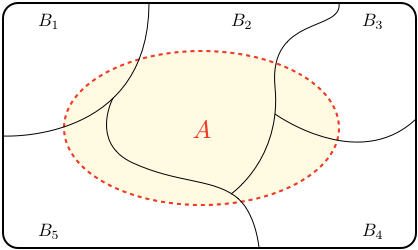
\includegraphics[scale=0.5]{total_prob.png}
    \end{center}
    \begin{align*}
        P(B) &= P(A_1B) + P(A_2B) + ... + P(A_nB) \\
             &= P(B|A_1)P(A_1) + P(B|A_2)P(A_2) + ... P(B|A_n)P(A_n) \\
             &= P(B) =  \sum_{i=1}^{n} P(B|A_i)P(A_i)
    \end{align*}

    \section{Combinatorics}

    Deals with counting, sampling, ordering, selection,\dots

    \subsection{Basic Concept of Counting}

    Combined number of outcomes: $m \times n \times k\dots$\\[\baselineskip]
    \textit{\textbf{Example:}} How many passwords can you create such 
    that the first two are small letters, next one is a capital letter, 
    and the last four are numbers?\\
    $$26\times 26\times 26\times 10\times 10\times 10\times 10 = N$$\\
    \textit{\textbf{Example:}} Given a hacker generates $10^8$ passwords (can be 
    repeated) what is the probability that at least one password will match yours?
    \begin{align*}
        P(passwordMatches) &= \frac{1}{N}\\
        P(passwordDoesNotMatch) &= 1 - \frac{1}{N}\\
        P(allPasswordsDoNotMatch) &= \left(1-\frac{1}{N}\right)^{10^8}\\
        P(atLeastOneMatch) &= 1 - \left(1-\frac{1}{N}\right)^{10^8}
    \end{align*}

    \subsection{Permutations}

    \textit{\textbf{Example:}} Suppose we have n distinguishable objects. 
    How many ways can you arrange the objects? (without replacement) 
    $$n!$$
    \textbf{with replacement}
    $$n^n$$
    Now suppose we are interested in choosing k objects out of n $(k \leq n)$, 
    \textbf{without replacement}; order is \textbf{important}
    $$n(n-1)(n-2)...(n-k+1)$$
    $$=\frac{n!}{(n-k)!}$$
    with replacement (given k terms)
    $$n(n)(n)...(n) = n^k$$
    \textit{\textbf{Example:}} You have a bookshelf with 4 math books, 
    3 physics, 2 economics, and 1 history book. How many ways can you arrange 
    the bookshelf such that similar books are bundled/adjancent?\\[\baselineskip]
    Ways of arranging the books:
    $$(4!)(3!)(2!)(1!)$$
    Now account for the ways you can arrange the bundles:
    $$(4!)(3!)(2!)(1!)(4!)$$
    \textit{\textbf{Example:}} Ways of creating a password of 
    5 numbers without replacement:
    $$\frac{10!}{(10-5)!}$$
    \textit{\textbf{Combination:}} How many ways can you select k 
    objects out of n distinguishable objects without replacement 
    (n choose k); order does \textbf{not} matter
    $$\frac{n!}{(n-k)!k!}$$
    represented as:
    $$\binom{n}{k}$$
    note that $\binom{n}{n-k}$ is the same thing\\[\baselineskip]
    \textit{\textbf{Example:}} Given a deck of cards, you choose 
    5 cards. What is the probability you get two aces?
    $$\frac{\binom{4}{2}\binom{48}{3}}{\binom{52}{5}}$$
    \textit{\textbf{Example:}} A team has 25 players, 15 are position 
    players, 10 are pitchers. The lineup consists of 9 players.
    \begin{enumerate}[label=(\alph*)]
        \item How many lineups can the manager create?\\
        $\binom{10}{1}\binom{15}{8} = \frac{(10)(15!)}{(7!)(8!)} = 64350$
        \item How many batting orders can he create?\\
        $64350(9!)$
    \end{enumerate}
    \textit{\textbf{Example:}} Suppose you pick 3 cards
    from a deck. What is the probability of getting at
    least an ace?
    \begin{align*}
        &= 1 - P(noAce)\\
        &= 1 - \frac{\binom{48}{3}}{\binom{52}{3}}
    \end{align*}
    \textit{\textbf{Example:}} Suppose you have 2 letters, A
    and B. How many sequences can you generate having 
    3 As and 5 Bs. 
    \begin{align*}
        &=\binom{8}{3} \times \binom{5}{5}\\
    \end{align*}
    \textit{\textbf{Example:}} You have 4 mailboxes and 8 
    indistinguishable balls. How many ways can you distribute
    the balls so that no box is empty. Let $x_1$ be the number of
    balls in box 1. We know $x_1+x_2+x_3+x_4 = 8$. $x_i$ is > 0 
    for all i. 
    $$- - - - - - - -$$
    Since there are 7 spaces, we choose three to split them up 
    in any box.\\
    Essentially
    $$\binom{n-1}{k-1}$$
    How many ways can you distribute the balls into the boxes. 
    A box can be empty.\\
    let $y_i = x_i + 1$ so\\
    $y_1+y_2+y_3+y_4 = 12$
    $$=\binom{11}{3}$$

    $$\sum_{k=0}^{n}\binom{n}{k} = \binom{n}{0} + \binom{n}{1} + ... + \binom{n}{n} = 2^n$$

    \subsection{Multinomial Coefficients}

    Suppose we have n distinguishable objects. We want to break them 
    into k groups. $G_1$ has $n_1$ objects, $G_2$ has $n_2$ objects,
    $G_k$ has $n_k$ objects. $n_1 + n_2 + ... + n_k = n$. How many ways
    can we do it?
    \begin{align*}
        &=\binom{n}{n_1}\binom{n-n_1}{n_2}\binom{n-n_1-n_2}{n_3}...\binom{n_1-...-n_{k-1}}{n_k}\\
        &= \frac{n!}{n_1!n_2!...n_k!}
    \end{align*}

    \section{Random Variables}

    A random variable (X) is a function mapping the outcomes of a random
    experiment into the real line. Mapping must be 1 to 1 \textit{or} many to 1.
    Mapping 1 to many is \textit{unacceptable}.

    \textit{\textbf{Example:}} Suppose you toss a coin twice. 
    $$\Omega = {HH, HT, TH, TT}$$
    X is a random variable as the number of heads. X can take the 
    value 0, 1, 2\\
    $$P(X=0) = \frac{1}{4}$$

    \subsection{Classification of Random Variables}

    Discrete, continuous, or mixed\\
    a R.V. is said to be discrete if it can take a finite or infinitely countable (i.e. integer values) number of values\\
    a R.V. is continuous if it can take infinitely uncountable number of values (i.e. real numbers) number of values\\
    \subsection*{How do we describe a discrete RV}
    PMF - probability mass function $P(X=k)$ for all possible values of k 
    $$\sum_{k}^{max}P(X=K) = 1$$
    CDF - Cumulative Distributive Function\\
    $$F_X(x) = P(X \leq x)$$
    Example: Suppose you toss a coin twice $\Omega = {HH, HT, TH, TT}$. Let $X =$ number of heads. HH to 2, HT to 1, TH -> 1, TT -> 0. 
    X is a disccrete RV taking on values of 0, 1, 2. Sketch the PMF and CDF.\\


\end{document}